

% Gradient Info
\tikzset {_fippvxhf7/.code = {\pgfsetadditionalshadetransform{ \pgftransformshift{\pgfpoint{0 bp } { 0 bp }  }  \pgftransformrotate{-70 }  \pgftransformscale{2 }  }}}
\pgfdeclarehorizontalshading{_3gd5tfphw}{150bp}{rgb(0bp)=(0.95,0.58,0.03);
rgb(47.66368865966797bp)=(0.95,0.58,0.03);
rgb(62.5bp)=(1,0.75,0.36);
rgb(100bp)=(1,0.75,0.36)}

\tikzset {_ny4acrtlv/.code = {\pgfsetadditionalshadetransform{ \pgftransformshift{\pgfpoint{0 bp } { 0 bp }  }  \pgftransformrotate{-70 }  \pgftransformscale{2 }  }}}
\pgfdeclarehorizontalshading{_s94vlkwi1}{150bp}{rgb(0bp)=(0.95,0.58,0.03);
rgb(47.66368865966797bp)=(0.95,0.58,0.03);
rgb(62.5bp)=(1,0.75,0.36);
rgb(100bp)=(1,0.75,0.36)}

\tikzset {_qee32nkz9/.code = {\pgfsetadditionalshadetransform{ \pgftransformshift{\pgfpoint{0 bp } { 0 bp }  }  \pgftransformrotate{-70 }  \pgftransformscale{2 }  }}}
\pgfdeclarehorizontalshading{_tehe75fq7}{150bp}{rgb(0bp)=(0.95,0.58,0.03);
rgb(47.66368865966797bp)=(0.95,0.58,0.03);
rgb(62.5bp)=(1,0.75,0.36);
rgb(100bp)=(1,0.75,0.36)}

\tikzset {_w8wh1nrda/.code = {\pgfsetadditionalshadetransform{ \pgftransformshift{\pgfpoint{0 bp } { 0 bp }  }  \pgftransformrotate{-70 }  \pgftransformscale{2 }  }}}
\pgfdeclarehorizontalshading{_vwajl3t91}{150bp}{rgb(0bp)=(0.95,0.58,0.03);
rgb(47.66368865966797bp)=(0.95,0.58,0.03);
rgb(62.5bp)=(1,0.75,0.36);
rgb(100bp)=(1,0.75,0.36)}

\tikzset {_4x4sblz9b/.code = {\pgfsetadditionalshadetransform{ \pgftransformshift{\pgfpoint{0 bp } { 0 bp }  }  \pgftransformrotate{-70 }  \pgftransformscale{2 }  }}}
\pgfdeclarehorizontalshading{_se3st60w5}{150bp}{rgb(0bp)=(0.95,0.58,0.03);
rgb(47.66368865966797bp)=(0.95,0.58,0.03);
rgb(62.5bp)=(1,0.75,0.36);
rgb(100bp)=(1,0.75,0.36)}

\tikzset {_nb9qk024g/.code = {\pgfsetadditionalshadetransform{ \pgftransformshift{\pgfpoint{0 bp } { 0 bp }  }  \pgftransformrotate{-70 }  \pgftransformscale{2 }  }}}
\pgfdeclarehorizontalshading{_pm53662fo}{150bp}{rgb(0bp)=(0.95,0.58,0.03);
rgb(47.66368865966797bp)=(0.95,0.58,0.03);
rgb(62.5bp)=(1,0.75,0.36);
rgb(100bp)=(1,0.75,0.36)}
\tikzset{every picture/.style={line width=0.75pt}} %set default line width to 0.75pt        

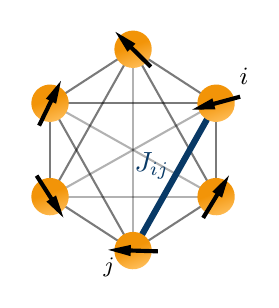
\begin{tikzpicture}[x=0.75pt,y=0.75pt,yscale=-1,xscale=1]

\draw [color={rgb, 255:red, 0; green, 0; blue, 0 }  ,draw opacity=0.52 ][line width=0.75]    (62.5,26.5) -- (102.5,52.5) ;
\draw [color={rgb, 255:red, 0; green, 0; blue, 0 }  ,draw opacity=0.52 ][line width=0.75]    (22.5,97.5) -- (62.5,123.5) ;
\draw [color={rgb, 255:red, 0; green, 0; blue, 0 }  ,draw opacity=0.52 ][line width=0.75]    (102.5,97.5) -- (62.5,123.5) ;
\draw [color={rgb, 255:red, 0; green, 0; blue, 0 }  ,draw opacity=0.52 ][line width=0.75]    (22.5,52.5) -- (22.5,97.5) ;
\draw [color={rgb, 255:red, 0; green, 0; blue, 0 }  ,draw opacity=0.52 ][line width=0.75]    (62.5,26.5) -- (22.5,52.5) ;
\draw [color={rgb, 255:red, 0; green, 0; blue, 0 }  ,draw opacity=0.52 ][line width=0.75]    (102.5,52.5) -- (102.5,97.5) ;
\draw [color={rgb, 255:red, 0; green, 0; blue, 0 }  ,draw opacity=0.3 ][line width=0.75]    (62.5,26.5) -- (62.5,123.5) ;
\draw [color={rgb, 255:red, 0; green, 0; blue, 0 }  ,draw opacity=0.52 ][line width=0.75]    (22.5,52.5) -- (62.5,123.5) ;
\draw [color={rgb, 255:red, 0; green, 0; blue, 0 }  ,draw opacity=0.52 ][line width=0.75]    (62.5,26.5) -- (22.5,97.5) ;
\draw [color={rgb, 255:red, 0; green, 0; blue, 0 }  ,draw opacity=0.52 ][line width=0.75]    (62.5,26.5) -- (102.5,97.5) ;
\draw [color={rgb, 255:red, 0; green, 0; blue, 0 }  ,draw opacity=0.3 ][line width=0.75]    (22.5,52.5) -- (102.5,97.5) ;
\draw [color={rgb, 255:red, 0; green, 0; blue, 0 }  ,draw opacity=0.52 ][line width=0.75]    (22.5,52.5) -- (102.5,52.5) ;
\draw [color={rgb, 255:red, 0; green, 0; blue, 0 }  ,draw opacity=0.3 ][line width=0.75]    (22.5,97.5) -- (102.5,97.5) ;
\draw [color={rgb, 255:red, 0; green, 0; blue, 0 }  ,draw opacity=0.3 ][line width=0.75]    (102.5,52.5) -- (22.5,97.5) ;
\draw [color={rgb, 255:red, 8; green, 57; blue, 102 }  ,draw opacity=1 ][line width=2.25]    (102.5,52.5) -- (62.5,123.5) ;
\draw  [draw opacity=0][shading=_3gd5tfphw,_fippvxhf7] (62.23,132.5) .. controls (57.26,132.35) and (53.35,128.2) .. (53.5,123.23) .. controls (53.65,118.26) and (57.8,114.35) .. (62.77,114.5) .. controls (67.74,114.65) and (71.65,118.8) .. (71.5,123.77) .. controls (71.35,128.74) and (67.2,132.65) .. (62.23,132.5) -- cycle ;
\draw [color={rgb, 255:red, 0; green, 0; blue, 0 }  ,draw opacity=1 ][line width=1.5]    (74.49,123.86) -- (54.5,123.26) ;
\draw [shift={(50.51,123.14)}, rotate = 1.72] [fill={rgb, 255:red, 0; green, 0; blue, 0 }  ,fill opacity=1 ][line width=0.08]  [draw opacity=0] (10.92,-2.73) -- (0,0) -- (10.92,2.73) -- cycle    ;

\draw  [draw opacity=0][shading=_s94vlkwi1,_ny4acrtlv] (104.86,61.19) .. controls (100.06,62.49) and (95.12,59.65) .. (93.81,54.86) .. controls (92.51,50.06) and (95.35,45.12) .. (100.14,43.81) .. controls (104.94,42.51) and (109.88,45.35) .. (111.19,50.14) .. controls (112.49,54.94) and (109.65,59.88) .. (104.86,61.19) -- cycle ;
\draw [color={rgb, 255:red, 0; green, 0; blue, 0 }  ,draw opacity=1 ][line width=1.5]    (114.08,49.36) -- (94.78,54.59) ;
\draw [shift={(90.92,55.64)}, rotate = 344.82] [fill={rgb, 255:red, 0; green, 0; blue, 0 }  ,fill opacity=1 ][line width=0.08]  [draw opacity=0] (10.92,-2.73) -- (0,0) -- (10.92,2.73) -- cycle    ;
\draw  [draw opacity=0][shading=_tehe75fq7,_qee32nkz9] (94.81,92.83) .. controls (97.39,88.58) and (102.92,87.23) .. (107.17,89.81) .. controls (111.42,92.39) and (112.77,97.92) .. (110.19,102.17) .. controls (107.61,106.42) and (102.08,107.77) .. (97.83,105.19) .. controls (93.58,102.61) and (92.23,97.08) .. (94.81,92.83) -- cycle ;
\draw [color={rgb, 255:red, 0; green, 0; blue, 0 }  ,draw opacity=1 ][line width=1.5]    (96.27,107.76) -- (106.65,90.66) ;
\draw [shift={(108.73,87.24)}, rotate = 121.28] [fill={rgb, 255:red, 0; green, 0; blue, 0 }  ,fill opacity=1 ][line width=0.08]  [draw opacity=0] (10.92,-2.73) -- (0,0) -- (10.92,2.73) -- cycle    ;
\draw  [draw opacity=0][shading=_vwajl3t91,_w8wh1nrda] (56.18,32.9) .. controls (52.64,29.41) and (52.6,23.71) .. (56.1,20.18) .. controls (59.59,16.64) and (65.29,16.6) .. (68.82,20.1) .. controls (72.36,23.59) and (72.4,29.29) .. (68.9,32.82) .. controls (65.41,36.36) and (59.71,36.4) .. (56.18,32.9) -- cycle ;
\draw [color={rgb, 255:red, 0; green, 0; blue, 0 }  ,draw opacity=1 ][line width=1.5]    (71.04,34.93) -- (56.81,20.88) ;
\draw [shift={(53.96,18.07)}, rotate = 44.64] [fill={rgb, 255:red, 0; green, 0; blue, 0 }  ,fill opacity=1 ][line width=0.08]  [draw opacity=0] (10.92,-2.73) -- (0,0) -- (10.92,2.73) -- cycle    ;
\draw  [draw opacity=0][shading=_se3st60w5,_4x4sblz9b] (14.41,48.56) .. controls (16.59,44.09) and (21.97,42.23) .. (26.44,44.41) .. controls (30.91,46.59) and (32.77,51.97) .. (30.59,56.44) .. controls (28.41,60.91) and (23.03,62.77) .. (18.56,60.59) .. controls (14.09,58.41) and (12.23,53.03) .. (14.41,48.56) -- cycle ;
\draw [color={rgb, 255:red, 0; green, 0; blue, 0 }  ,draw opacity=1 ][line width=1.5]    (17.24,63.29) -- (26,45.31) ;
\draw [shift={(27.76,41.71)}, rotate = 115.98] [fill={rgb, 255:red, 0; green, 0; blue, 0 }  ,fill opacity=1 ][line width=0.08]  [draw opacity=0] (10.92,-2.73) -- (0,0) -- (10.92,2.73) -- cycle    ;
\draw  [draw opacity=0][shading=_pm53662fo,_nb9qk024g] (30.09,92.66) .. controls (32.76,96.85) and (31.53,102.41) .. (27.34,105.09) .. controls (23.15,107.76) and (17.59,106.53) .. (14.91,102.34) .. controls (12.24,98.15) and (13.47,92.59) .. (17.66,89.91) .. controls (21.85,87.24) and (27.41,88.47) .. (30.09,92.66) -- cycle ;
\draw [color={rgb, 255:red, 0; green, 0; blue, 0 }  ,draw opacity=1 ][line width=1.5]    (16.04,87.39) -- (26.81,104.24) ;
\draw [shift={(28.96,107.61)}, rotate = 237.44] [fill={rgb, 255:red, 0; green, 0; blue, 0 }  ,fill opacity=1 ][line width=0.08]  [draw opacity=0] (10.92,-2.73) -- (0,0) -- (10.92,2.73) -- cycle    ;

\draw (61.7,74.8) node [anchor=north west][inner sep=0.75pt]  [color={rgb, 255:red, 8; green, 57; blue, 102 }  ,opacity=1 ]  {$J_{ij}$};
\draw (112.4,34.13) node [anchor=north west][inner sep=0.75pt]  [font=\small,color={rgb, 255:red, 0; green, 0; blue, 0 }  ,opacity=1 ]  {$i$};
\draw (46.8,125.73) node [anchor=north west][inner sep=0.75pt]  [font=\footnotesize,color={rgb, 255:red, 0; green, 0; blue, 0 }  ,opacity=1 ]  {$j$};

\end{tikzpicture}